\documentclass[11pt]{article}
\usepackage[margin=2cm,bottom=2cm]{geometry}
\usepackage[utf8]{inputenc}
\usepackage{mathtools}
\usepackage{hyperref}
\usepackage{ragged2e}
\usepackage{tocloft}
\linespread{1.3}
\setcounter{secnumdepth}{5}
\setcounter{tocdepth}{5}

\usepackage[T1]{fontenc}    % this is needed for correct output of umlauts in pdf
\usepackage{listings} % needed for the inclusion of source code
\usepackage{color}
\usepackage[table]{xcolor}
\usepackage{xcolor,colortbl}
%\usepackage{fourier}
\usepackage[math]{iwona}
\usepackage[T1]{fontenc}
\usepackage{makecell}
\usepackage{graphicx}
\usepackage{wasysym}
\newcommand*{\vimage}[1]{\vcenter{\hbox{\includegraphics[scale=0.1]{#1}}}}
\newcommand*{\vimaged}[1]{\vcenter{\hbox{\includegraphics[scale=0.12]{#1}}}}
\newcommand*{\vpointer}{\vcenter{\hbox{\scalebox{2}{\Huge\pointer}}}}

\renewcommand\theadalign{cb}
\renewcommand\theadfont{\bfseries}
\renewcommand\theadgape{\Gape[6pt]}
\renewcommand\cellgape{\Gape[6pt]}

\newcommand{\mc}[2]{\multicolumn{#1}{c}{#2}}

\definecolor{LightCyan}{rgb}{0.88,1,1}
\definecolor{mavi}{rgb}{0,0.1568,0.3019}
\definecolor{dkgreen}{rgb}{0,0.6,0}
\definecolor{gray}{rgb}{0.5,0.5,0.5}
\definecolor{mauve}{rgb}{0.58,0,0.82}
\definecolor{backcolour}{rgb}{0.95,0.95,0.92}

\definecolor{gray}{rgb}{0.4,0.4,0.4}
\definecolor{backcolour}{rgb}{0.97,0.97,0.97}
\lstset{language=Java,                 
  basicstyle={\footnotesize\ttfamily} ,
  numbers=left,                   
  numberstyle=\tiny\color{gray},  
  stepnumber=1,
  numbersep=5pt,                  
  backgroundcolor=\color{backcolour}, 
  showspaces=false,               
  showstringspaces=false,         
  showtabs=false,                 
  %frame=single,               
  rulecolor=\color{black},        
  tabsize=4,                     
  captionpos=b,                   
  breaklines=true,                
  breakatwhitespace=true,        
  title=\lstname,                 
                                  % also try caption instead of title
  %keywordstyle=\color{blue},          % keyword style
  commentstyle=\color{gray},       % comment style
  %stringstyle=\color{mauve},         % string literal style
  escapeinside={\%*}{*)},            % if you want to add a comment within your code
  morekeywords={*,...}  
} 

\renewcommand{\cftsecleader}{\cftdotfill{\cftdotsep}}

\begin{document}
\begin{titlepage}

\newcommand{\HRule}{\rule{\linewidth}{0.5mm}} 

\begin{figure}

\includegraphics[width=0.77\textwidth]{bilgi.jpg}
\end{figure}

\center 

\textsc{\LARGE}\\[0.3cm]
\textsc{\LARGE Istanbul Bilgi University}\\[1.2cm]
\textsc{\Large Faculty Of Engineering}\\[0.5cm]
\textsc{\large Computer Engineering}\\[0.7cm] 

\HRule \\[0.8cm]
{ \huge \bfseries Bluetooth - WIFI Communication Car}\\[0.4cm] 
\HRule \\[0.8cm]
 
\begin{minipage}{0.4\textwidth}
\begin{flushleft} \large
\centering
\vspace{0.7cm}
\emph{\textbf{By:}}\\
Mehmetcan Güleşçi - 112200032 \\
\vspace{1cm}
\emph{\textbf{Supervised by:}}\\
Yrd. Doç Dr. Murat Orhun
\end{flushleft}
\end{minipage}

\begin{minipage}{0.4\textwidth}
\end{minipage}\\[2cm]

\vspace{1.75cm}
{\large \today}\\[2cm]


\vfill
\end{titlepage}

\pagebreak

\tableofcontents
\vspace{1cm}
\listoffigures
\addcontentsline{toc}{section}{List of Figures}
\listoftables
\addcontentsline{toc}{section}{List of Tables}

\pagebreak

%%%%%%%%%%%%%%%%%%%%%%%%%%%%%%%%%%%%%%%%%%%%%%%%%%
% SECTION
%%%%%%%%%%%%%%%%%%%%%%%%%%%%%%%%%%%%%%%%%%%%%%%%%%
\section{Abstract}
\begin{flushleft}
As we known, mobile platform has become a limb which all humanity from young to old cannot give up. Therefore, it is the case that an application made on this platform will be more interesting, enjoyable and more useful for them.\\
\vspace{0.2cm}
The development of smartphones offers a preliminary opportunity for low cost robots. Some of them are the WIFI, Bluetooth and camera systems which will be used in the project. Besides, it has a stronger CPU. This means that it expresses speed in terms of data communication.\\
\vspace{0.2cm}
In this project, Android supported device is used as a robot brain. At this point, it is possible to talk about two kinds of communication. One of these is the communication between our WIFI Module and the smartphone, the other one is on the basic Android application which we will use and Arduino with serial communication. When we consider these things, my first aim is to be able to command and control the Robot by using Bluetooth, the second one is to be able to taking live view from the camera by using WIFI Module. This was a simple abstract for this projects. These details will be discussed in this report clearly.
\end{flushleft}

\vspace{0.5cm}

%%%%%%%%%%%%%%%%%%%%%%%%%%%%%%%%%%%%%%%%%%%%%%%%%%
% SECTION
%%%%%%%%%%%%%%%%%%%%%%%%%%%%%%%%%%%%%%%%%%%%%%%%%%
\section{Introduction}
\begin{flushleft}
A benefit of having a Bluetooth connection is that the establishment of the connection will be automatic once the device is paired with the Bluetooth node in the car. Another advantage with the Bluetooth technology is that it is an open standard, which means that if the Bluetooth devices all follow this standard they should be compatible with each other. Other advantages with the Bluetooth technology that are especially good for the car environment are the small
physical size and the small power consumption.\\
\vspace{0.2cm}
In this way, we can say that it is possible to control a robot using a Bluetooth connection. The Bluetooth module in our robotic car will be connected to the L298P Motor Shield attached to the Arduino. In this system, the person who will manage the robot is the user who will use the phone. When the user sends control signals using the forward, backward, left and right buttons via android phones, these signals will be transmitted by Bluetooth and captured the current view from the HD Camera by using WIFI module which will be mounted on the robot. This signal will be transmitted to the controller which is connected to it so to the Arduino via the Motor driver shield. These controllers will analyze the signal. The robot will be moved according to the forward, backward, right, left commands which is sent by the user via Android. For this reason it will be possible to move the robot on four sides.\\
\vspace{0.2cm}
As a result, this project will be provided by two communication Bluetooth, WIFI. Thanks to Bluetooth, motion will be provided. The camera which is mounted on robot will capture the live video from WIFI and send it to the Android user. This will give the current position of the robot. Based on that video we can determine whether we need to move the robot forward, backward, right or left.
\end{flushleft}

\pagebreak

\begin{center}
\begin{table}
\begin{tabular}{ |c| c | c | c | c |}
\hline
\thead{From/To \\ Android} & \thead{From/To \\ HD Camera} & \thead{On \\ WIFI Module} & \thead{On - From/To \\ Motor Shield (UNO R3)} & \thead{On \\ Bluetooth}\\ \hline

\makecell{Signal to Android \\ from HD Cam (1)} &  \makecell{Signal from HD Cam \\ to Android (2)}  & \color{mavi}\Huge $\bullet$ & \color{mavi}\Huge $\bullet$ &   \\ \hline

\makecell{Signal from Android \\ to Motor Shield (3)} &    &  & \makecell{Signal to Motor Shield \\ from Android (4)} & \color{mavi}\Huge $\bullet$   \\ \hline
\end{tabular}
\caption{Communication Tables}
\end{table}
\end{center}

\subsection{Communication Between Devices}
\begin{flushleft}
\hspace{0.5cm}When we look at the table above:\\
\begin{itemize}
\item[1] To get Cam view from HD Cam on WIFI Module (to take IP) and Motor Shield (in terms of power).
\item[2] To send Cam view to Android.
\item[3] To send button motion to motor.
\item[4] To get button motion from Android on Bluetooth
\end{itemize}
\end{flushleft}

\vspace{0.4cm}

\subsection{Objectives}
\begin{itemize}
\item To enable inserting Arduino Code to give first motion to the car.
\item To enable Android buttons to control the car as remoted.
\item To enable getting live view on the HD Cam by using WIFI Module and display the robot eyes on Android Screen.
\end{itemize}

%%%%%%%%%%%%%%%%%%%%%%%%%%%%%%%%%%%%%%%%%%%%%%%%%%
% SECTION
%%%%%%%%%%%%%%%%%%%%%%%%%%%%%%%%%%%%%%%%%%%%%%%%%%
\pagebreak
\section{Processes of Car}
\begin{flushleft}
I want to examine the car’s processes in two parts. One of them is primarily hardware. The hardware side will include the controller cards that will be used in our remote controlled car, what they are and their detailed features.\\
\vspace{0.2cm}
The other part is the software that will give the necessary action to the car. I will include to this section in second semester. Now we will talk about hardware.
\end{flushleft}

\vspace{0.3cm}

\subsection{Hardware Parts}
\subsubsection{Requirements}
\begin{flushleft}
I have tried to show the modules for motors which are necessary for their working mechanism and their numbers within the scope of this project on the table below.
\vspace{0.2cm}
\end{flushleft}
\begin{table}[h]
\centering 
\begin{tabular}{|c|c|}
 \hline
 \textbf{\emph{\cellcolor{red!27}Number}} & \textbf{\emph{\cellcolor{red!27}Needed}}	\\ [0.5ex] \hline
 1 & UNO R3 \\  \hline
 1 & L298P Motor Shield \\  \hline
 1 & Digital WIFI Module \\  \hline
 1 & HD Camera \\  \hline
 1 & HC05 Bluetooth Module \\ \hline
 1 & DC Motors \\
 \hline
\end{tabular}
\caption{Requirements}
\label{table:1}
\end{table}

\begin{flushleft}
Now I want to talk about these pieces. What are they? What do they do?
\end{flushleft}

\vspace{0.3cm}

\paragraph{Arduino UNO R3}
\subparagraph*{What is Arduino ?}
\addcontentsline{toc}{subparagraph}{What is Arduino ?}
\begin{flushleft}
We can think of it as an electronic unit like our brain, like our computer’s processor. This unit is a microcontroller that makes what you want when you want it, or controls physical inputs with various sensors and converts these inputs into the desired output. Thanks to sensors and activators which are connected to Arduino, you can do whatever you want. By connecting the Arduino to our computer we can view the sensor data and transactions and control the equipment from the computer. This requires only a little electronic knowledge a
little programming knowledge.\\
\vspace{0.2cm}
\begin{figure}[h]
\centering
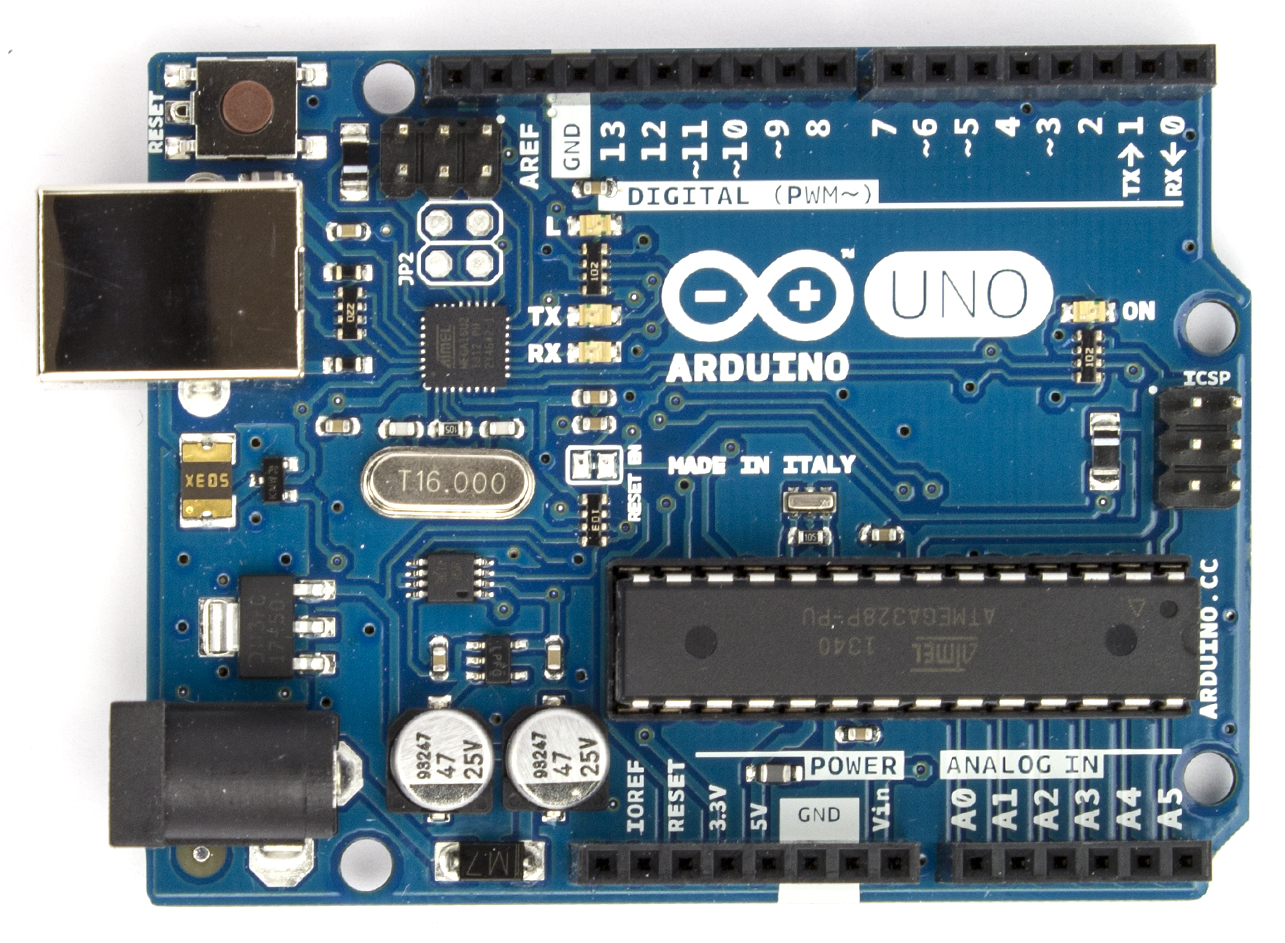
\includegraphics[scale=.25]{arduino.png}
\caption{Arduino Uno R3}
\end{figure}
\vspace{0.2cm}
Arduino which is an open source electronic development environment spreads rapidly. This software is a combination of language C ++ and Java languages and provides us with many advantages and convenience. Writing a program with Arduino is simpler and thanks to the built-in interface you can develop the program without difficulty in the Arduino programming language.
\end{flushleft}

\vspace{0.1cm}
\subparagraph*{Other features that highlight Arduino’s from other development environments}
\addcontentsline{toc}{subparagraph}{Other features that highlight Arduino’s from other development environments}
\begin{itemize}
\item Easy to use.
\item Communicating with everything by following various methods (computer, television, internet, GPS, loudspeaker, sensors, smart phones, cameras, motors ...).
\item Rich library support and many example applications.
\item Ideal for prototyping
\end{itemize}

\pagebreak

\begin{figure}[h]
\centering
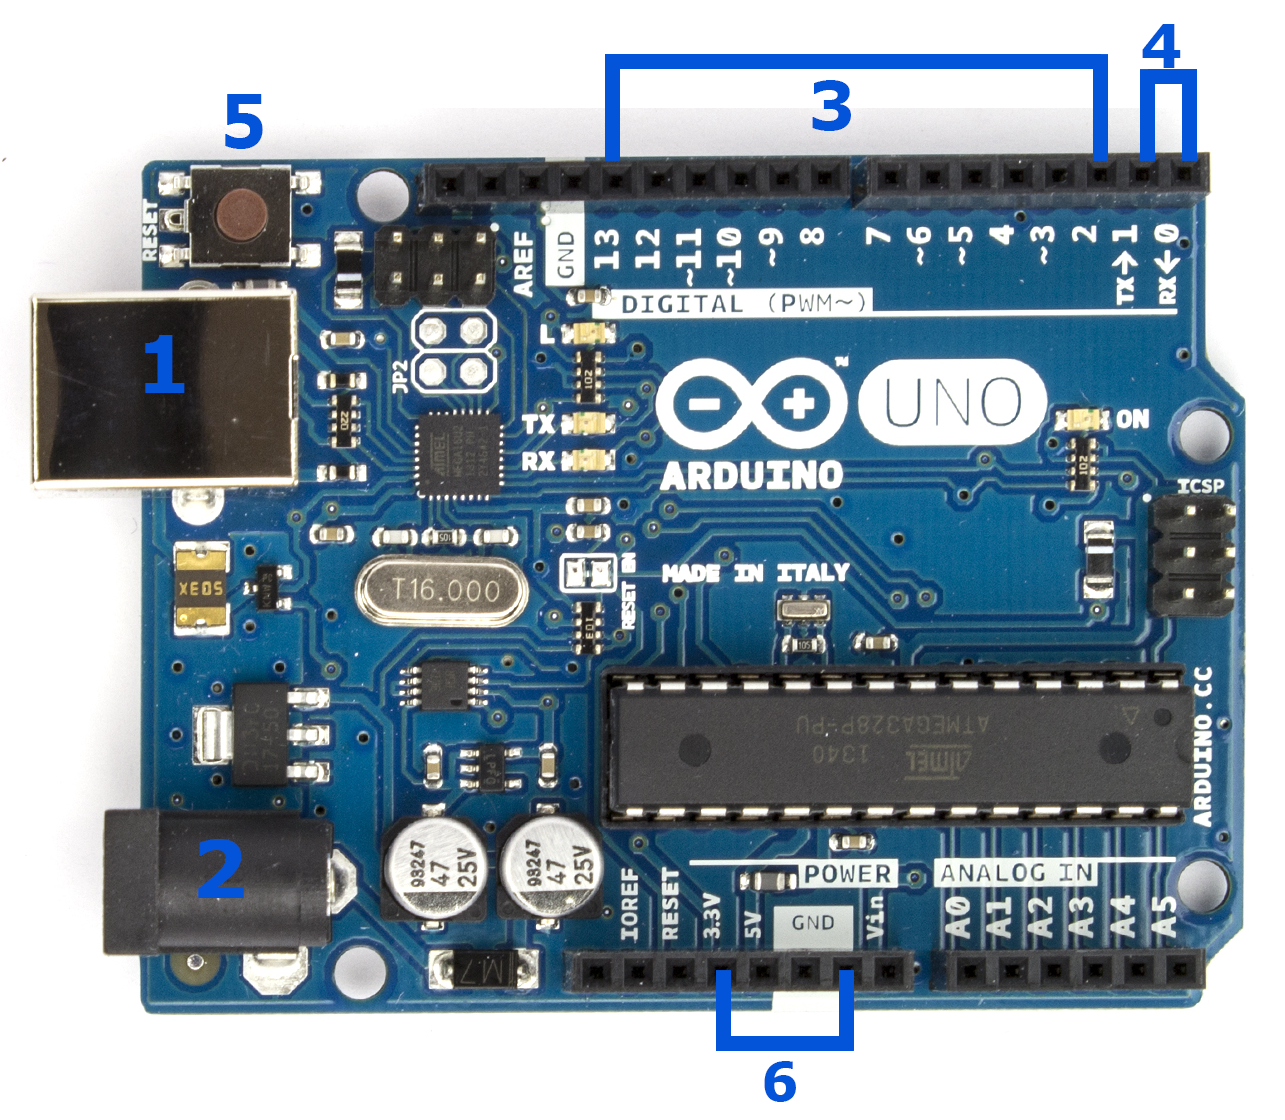
\includegraphics[scale=0.25]{arduinoreview.png}
\caption{Arduino detailed Review}
\end{figure}

\subparagraph*{Power}
\addcontentsline{toc}{subparagraph}{Power}
\begin{itemize}
\item[] \textbf{(1) USB:} We can send the code to the Arduino board thanks to it.
\item[] \textbf{(2):} Known as Arduino’s external power supply (7-12V)
\item[] \textbf{VIN:} The voltage input used when an external power supply is connected to the Arduino Uno card.
\item[] \textbf{(6) 5V:} This pin provides 5 V output from the regulator on the Arduino board. The card can be powered from the DC
power jack (part 2) with a 7-12 V adapter, 5 V from the USB jack (part 1) or 7-12 V from the VIN pin. The voltage supply from the 5V and 3.3V pins disregards the regulator and damages the card.
\item[] \textbf{(6) 3.3V:} The 3.3V output from the regulator on the Arduino card. The maximum is 50mA.
\item[] \textbf{(6) GND:} Ground pin.
\end{itemize}

\vspace{0.1cm}

\subparagraph*{Inputs and Outputs}
\addcontentsline{toc}{subparagraph}{Inputs and Outputs}
\begin{itemize}
\item[] All 14 digital input / output pins in Arduino Uno can be used as input or output with pinMode (), digitalWrite () and digitalRead () functions. These pins work with 5V.
\item[] \textbf{(4) 0(RX) - 1(TX):} These pins to receive data (receive - RX) and transmit (transmit - TX).
\item[] \textbf{(3) PWM 3, 5, 6, 9, 10, and 11:} These pins provide an 8-bit PWM signal with the analogWrite () function.
\item[] \textbf{(5) RESET:} To reset the microcontroller. It is usually used to add a reset button on the shield.
\end{itemize}

\pagebreak

\paragraph{L298P Motor Shield}
\begin{flushleft}
L298P Motor Drive integration is a full-bridge motor driver based on Arduino Uno. It can drive two separate 2A DC motors or one 2A stepper motor. It can be directly plugged into the Arduino.
\end{flushleft}
\begin{figure}[h]
\centering
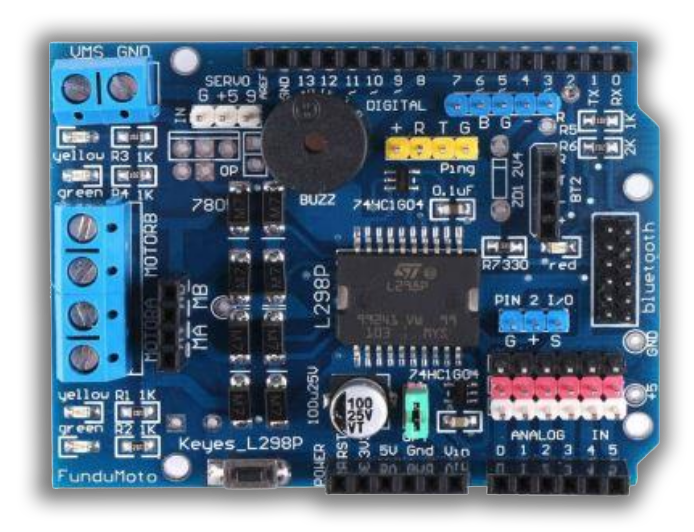
\includegraphics[scale=0.30]{l298.png}
\caption{L298P Motor Shield}
\end{figure}

\subparagraph*{Features}
\addcontentsline{toc}{subparagraph}{Features}
\begin{itemize}
\item Take Arduino's data.
\item On board buzzer (D4), you can set the astern alarm ringtone.
\item Convenient motor interface can be two routes motor output.
\item Two-way Bluetooth interface requires no wiring and you can plug directly.
\item It has six analog interfaces (A0, A1, A2, A3, A4, and A5).
\item It has seven digital interface that are not occupied (including D2, D3, D5, D6, D7, D8, and D9).
\end{itemize}
\begin{figure}[h]
\centering
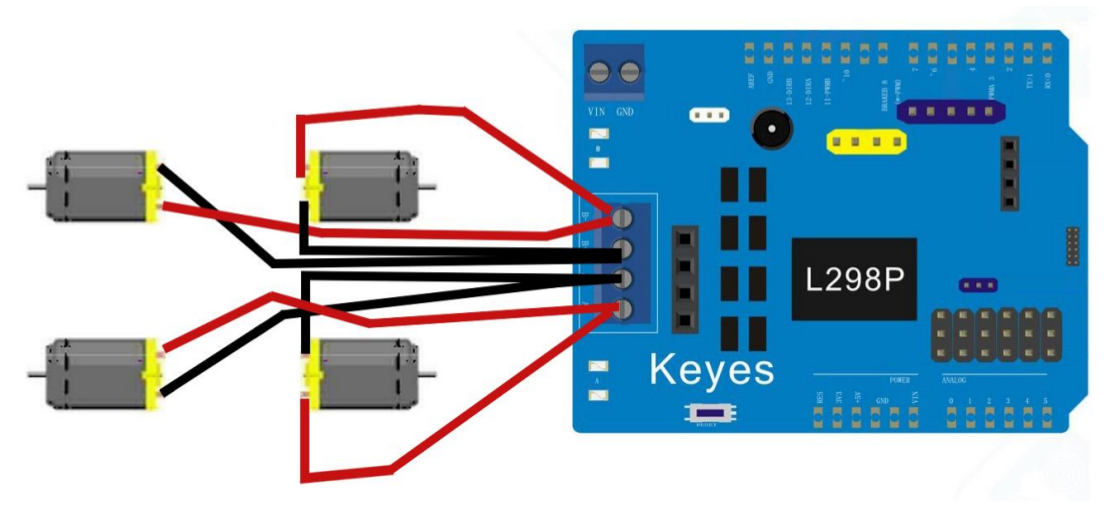
\includegraphics[scale=0.30]{connectl298.png}
\caption{Connect L298P to DC Motors}
\end{figure}

\vspace{0.1cm}

\subparagraph*{Technical Specifications}
\addcontentsline{toc}{subparagraph}{Technical Specifications}
\begin{itemize}
\item Operating Voltage: 5V-12V
\item L298P Motor Controller: Drive 2 separate DC motors or 1 step motor
\item Max. Current: Per 2A channel (with external supply)\\
\end{itemize}
\begin{flushleft}
Speed control function are connected with the 10, 11 interfaces. Direction control function are connected with the 12, 13 interfaces. And buzzer (alarm) function is expressed with the 4 interface. This is shown as the following table:
\end{flushleft}
\begin{table}[h]
\centering 
\begin{tabular}{|c|c|c|}
 \hline
 \textbf{\emph{\cellcolor{red!27}Function}} & \textbf{\emph{\cellcolor{red!27}Channel A Pin}} & \textbf{\emph{\cellcolor{red!27}Channel B Pin}}	\\ [0.5ex] \hline
 Direction & D12 & D13 \\  \hline
 PWM & D10 & D11\\ 
 \hline
\end{tabular}
\caption{Shield pin usage table}
\label{table:1}
\end{table}

\vspace{0.2cm}

\paragraph{Digital WIFI Module}
\begin{itemize}
\item Thanks to this card, our Android application will be connected to Cam
port thanks to IP which is in this module (may be 192.168.1.1).
\item The usb input on it allows us to connect our HD Cam.
\end{itemize}
\begin{figure}[h]
\centering
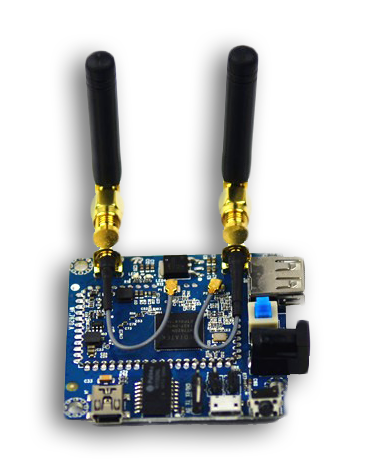
\includegraphics[scale=0.35]{wifi.png}
\caption{Digital WIFI Module}
\end{figure}

\pagebreak

\begin{itemize}
\item The cables from the WIFI Module are connected to the relevant parts of the L298P Motor Shield which is integrated on the Arduino. (Just to provide a power etc. GND-5V )
\item The connection will be provided to android phone on the
WIFI Module's IP address.
\end{itemize}
\begin{figure}[h]
\centering
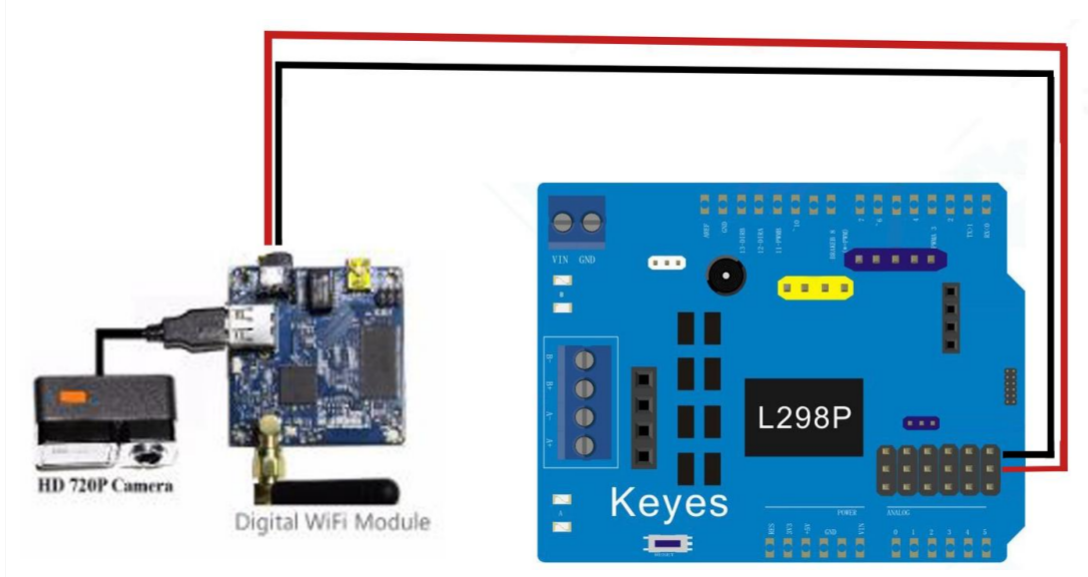
\includegraphics[scale=0.35]{connectwifi.png}
\caption{Digital WIFI Module and L298P Motor Shield}
\end{figure}

\vspace{0.2cm}

\paragraph{HD Camera}
\begin{flushleft}
It will be possible to transfer live video to the phone with the HD camera when the necessary operation is done thanks to the usb connection which is connected to WIFI Module.
\end{flushleft}
\vspace{0.3cm}
\begin{figure}[h]
\centering
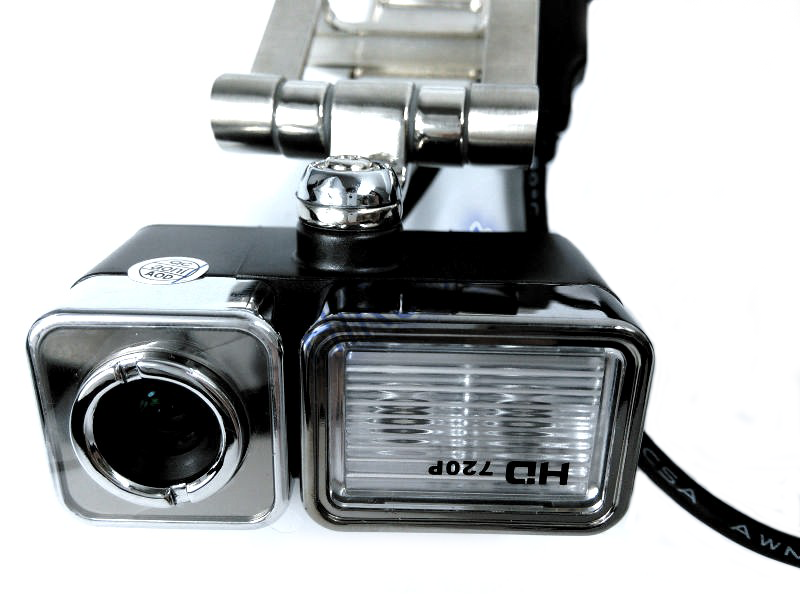
\includegraphics[scale=0.25]{camtemiz.png}
\caption{HD Cam}
\end{figure}

\pagebreak

\paragraph{Bluetooth Module}
\begin{flushleft}
There are 4 pins on VCC, GND, Rx and Tx on the Bluetooth module. From these VCC and GND are used to feed the Uno module. This project will be designed as sending data to Bluetooth module when certain button pressed from user. The Bluetooth module on Arduino receives the data and send to Arduino through the TX pin of Bluetooth module (RX pin of Arduino).
\end{flushleft}
\begin{figure}[h]
\centering
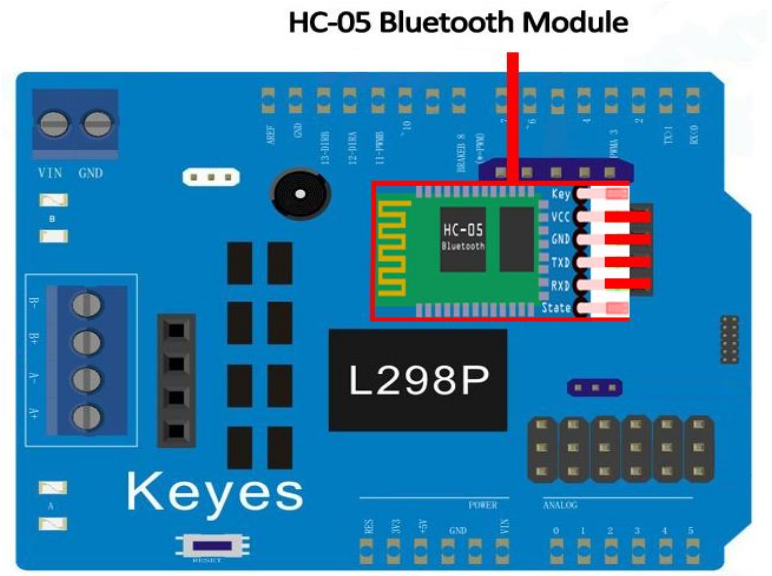
\includegraphics[scale=0.30]{blue.png}
\caption{Bluetooth Module on L298P}
\end{figure}

\vspace{0.2cm}

\paragraph{DC Motors}
\begin{flushleft}
The most preferred type of motor in robotics is DC motors. DC motors are cheap, small and effective. They are also very various in terms of size, shape and power. These are another reason to use them. Now we will explain dc motors in terms of direction, speed, voltage and current.
\end{flushleft}
\begin{itemize}
\item[] \textbf{\textit{Direction:}} When a power supply is connected to the DC motors, the direction of rotation of the DC motor depends on the direction of the current. When the direction of the current is reversed, the direction of rotation of the DC motor is reversed.

\item[] \textbf{\textit{Speed:}} The speed of a motor is measured by the number of revolutions completed in a minute. The
speed of the motor depends on the voltage and the load.
\end{itemize}

\begin{figure}[h]
\centering
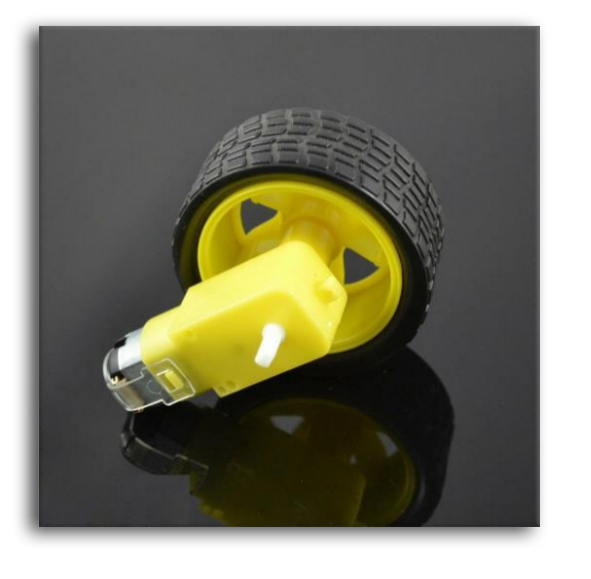
\includegraphics[scale=0.4]{dcmotor.png}
\caption{Dc Motor}
\end{figure}
\pagebreak
\begin{itemize}
\item[] \textbf{\textit{Voltage:}} Small DC motors can be found with voltage values ranging from 1.5 V to 48 V. While using DC motors in robots and other systems, this voltage value is important because it determines the maximum operating voltage to be applied to the DC motor.

\item[] \textbf{\textit{Current:}} When a DC motor is operated at the specified voltage, the current of the DC motor depends on the load. If the load increases, the current by the DC motor increases. The DC motor should not be overloaded to exceed the maximum current limit. In such a case, the DC motor is short-circuited and the applied power turns into heat. This may cause the DC motor to burn for long periods of time. Generally,the applied current range of DC motors can be up to 50mA and above 2A.
\end{itemize}

\pagebreak

\subsubsection{Car Building Process}
\begin{flushleft}
On the hardware side, the first step is to mount the dc motors which are wired, to the chassis.
\end{flushleft}
\begin{center}
$\vimaged{chasises1.png}\vpointer\vimaged{dc_motors1.png}\vpointer\vimaged{motorsfinal.png}$
\end{center}
\vspace{0.15cm}
\begin{flushleft}
The second step is to connect the dc motors to the motor driver shield. The third step is to mount the wifi shield on the chassis.
\end{flushleft}
\begin{center}
$\vimaged{shield_chasis.png}\vpointer\vimaged{shield_wifi_chasis.png}$
\end{center}
\vspace{0.15cm}
\begin{flushleft}
The fourth step is to connect the HD Camera to the chassis. In the fifth step, the wheels are finally mounted and the car is ready.
\end{flushleft}
\begin{center}
$\vimaged{shield_wifi_cam_chasis}\vpointer\vimaged{shield_wifi_wheels_chasis}$
\end{center}

\pagebreak

\subsection{Software Parts}
\subsubsection{Arduino Programming Language}
\begin{flushleft}
The open-source Arduino Software (IDE) makes it easy to write code and upload it to the board. The environment is written in Java and based on Processing and other open-source software.  This software can be used with any Arduino board. 
\end{flushleft}
\vspace{0.2cm}
\begin{figure}[h]
\centering
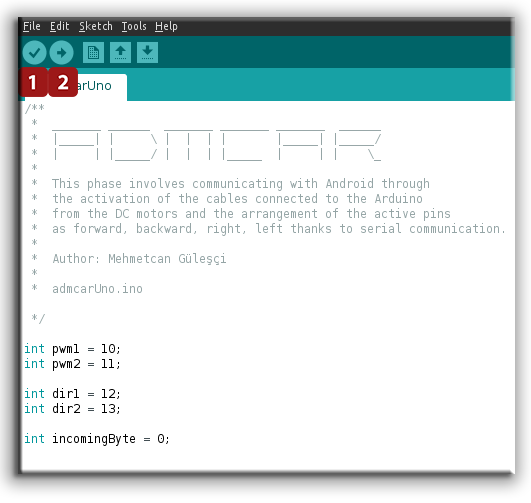
\includegraphics[scale=0.6]{update_execute.png}
\caption{Arduino Usage}
\end{figure}
\vspace{0.2cm}
\begin{itemize}
\item[1.] It allows us to check the Arduino code for errors.
\item[2.] It allows us to execute our Arduino code and upload to board.
\end{itemize}
\vspace{0.2cm}

\pagebreak

\paragraph*{Arduino Code}
\begin{flushleft}
All my arduino codes for this project is shown below.
\end{flushleft}
\begin{lstlisting}
/**
 *  _______ ______  _______ _______ _______  ______
 *  |_____| |     \ |  |  | |       |_____| |_____/
 *  |     | |_____/ |  |  | |_____  |     | |    \_
 * 
 *  This phase involves communicating with Android through 
 *  the activation of the cables connected to the Arduino 
 *  from the DC motors and the arrangement of the active pins 
 *  as forward, backward, right, left thanks to serial communication.
 * 
 *  Author: Mehmetcan Gulesci
 * 
 *  admcarUno.ino
                                                
 */
 
// Initialize variables
int pwm1 = 10;
int pwm2 = 11;

int dir1 = 12;
int dir2 = 13;

int incomingByte = 0;

/*  The setup() function is called when a sketch starts. Use it to initialize 
 *  variables, pin modes, start using libraries, etc. The setup function will 
 *  only run once, after each powerup or * reset of the Arduino board.
 */

void setup()
{
  pinMode(pwm1, OUTPUT);
  pinMode(pwm1, OUTPUT);
  pinMode(dir1, OUTPUT);
  pinMode(dir2, OUTPUT);

  digitalWrite(pwm1, LOW);
  digitalWrite(pwm2, LOW);
  digitalWrite(dir1, LOW);
  digitalWrite(dir2, LOW);

  Serial.begin(9600);
}

// This was my method to call digitalWrite- analogWrite functions in merged file
void MotorKontrol(int mdir1, int mdir2, int pwmSpeed)
{
  digitalWrite(dir1, mdir1);
  digitalWrite(dir2, mdir2);
  analogWrite(pwm1, pwmSpeed);
  analogWrite(pwm2, pwmSpeed);
}

void loop()
{
  // This expresses the motion part with serial communication
  if (Serial.available() > 0)
  {
    incomingByte = Serial.read();

    if (incomingByte == 10) // Forward
    {
      MotorKontrol(HIGH, HIGH, 170);
    }
    else if (incomingByte == 20) // Backward
    {
      MotorKontrol(LOW, LOW, 170);
    }
    else if (incomingByte == 30) // Left
    {
      MotorKontrol(HIGH, LOW, 170);
    }
    else if (incomingByte == 40) // Right
    {
      MotorKontrol(LOW, HIGH, 170);
    }
    else // Stop if another data comes
    {
      MotorKontrol(LOW, LOW, 0);
    }
  }
}
\end{lstlisting}

\pagebreak

\subsubsection{Android IDE}
\paragraph{Android Application All Part of Code}
\begin{flushleft}
This field contains everything from the birth to the end of the Android App. The design consists of 3 separate layouts.
\end{flushleft}
\begin{itemize}
\item \verb|activity_intro.xml|
\item \verb|activity_bluetooth_list.xml|
\item \verb|activity_car.xml|
\end{itemize}
\vspace{0.1cm}
\begin{flushleft}
$\succ$ As we know, each screen designed in layout includes its own software. So it is necessary to open the class at least as much as it is. The first of these is the \verb|SplashActivity.java| class, which corresponds to the \verb|activity_intro.xml| layout.When we open the app , we encounter this activiy first time, and it goes to the main layout with the transition time of 3 seconds. 
\end{flushleft}
\vspace{0.1cm}
\begin{lstlisting}
package com.example.mgulesci.admcar;

import android.content.Intent;
import android.os.Bundle;
import android.support.v4.app.FragmentActivity;

/**
 * This class refers to intro screen of my application
 */
public class SplashActivity extends FragmentActivity {
    public Thread myThread;

    @Override
    protected void onCreate(Bundle savedInstanceState) {
        super.onCreate(savedInstanceState);
        setContentView(R.layout.activity_intro);

        myThread = new Thread() {
            @Override
            public void run() {
                try {
                    sleep(3000);
                    // Open new intent after elapsed time
                    Intent intent = new Intent(getApplicationContext(), BluetoothList.class);
                    startActivity(intent);
                    finish();
                } catch (InterruptedException e) {
                    e.printStackTrace();
                }
            }
        };
        myThread.start();
    }
}
\end{lstlisting}

\begin{flushleft}
$\succ$ The second of these is the \verb|BluetoothList.java| class, which corresponds to the \verb|activity_bluetooth_list.xml| layout. The first thing to do in this class is to see the bluetooth feature of the phone and to see the bluetooth paired devices with the adapter methods on related layout.
\end{flushleft}
\vspace{0.1cm}
\begin{lstlisting}
package com.example.mgulesci.admcar;

import android.bluetooth.BluetoothAdapter;
import android.bluetooth.BluetoothDevice;
import android.content.Intent;
import android.os.Bundle;
import android.support.v4.app.FragmentActivity;
import android.view.View;
import android.widget.AdapterView;
import android.widget.ArrayAdapter;
import android.widget.Button;
import android.widget.ListView;
import android.widget.TextView;
import android.widget.Toast;

import java.util.ArrayList;
import java.util.Set;


public class BluetoothList extends FragmentActivity {

    public static String EXTRA_ADDRESS = "device_address";
    private TextView text;
    private ListView listOfDevices;
    private Button btn_list;
    private BluetoothAdapter phoneBluetooth = null;
    private Set<BluetoothDevice> pairedDevices;

    @Override
    protected void onCreate(Bundle savedInstanceState) {
        super.onCreate(savedInstanceState);
        setContentView(R.layout.activity_bluetooth_liste);

        this.initializeComponents();
        this.bluetoothControl();
        this.initializeListeners();

    }

    /**
     * Control the bluetooth whether it exists or not.
     */
    private void bluetoothControl(){
        // Take our phone's bluetooth
        phoneBluetooth = BluetoothAdapter.getDefaultAdapter();

        // Control, if your phone has bluetooth or not
        if (phoneBluetooth == null) {
            // If bluetooth is not available, give warning message and close application
            message("Your phone does not support bluetooth");
            finish();
        } else if (!phoneBluetooth.isEnabled()) {
            // If you have a bluetooth but it is not open, request to connect.
            Intent BTac = new Intent(BluetoothAdapter.ACTION_REQUEST_ENABLE);
            startActivityForResult(BTac, 1);
        }
    }

    /**
     * Initialize the components
     */
    private void initializeComponents(){
        // Describing XML Widgets
        text = (TextView) findViewById(R.id.textView);
        listOfDevices = (ListView) findViewById(R.id.listView);
        btn_list = (Button) findViewById(R.id.ButtonTest);
    }

    /**
     * Initialize the listeners
     */
    private void initializeListeners(){
        btn_list.setOnClickListener(new View.OnClickListener() {
            @Override
            public void onClick(View v) {
                showPairedDevices();
            }
        });
    }

    /**
     * This method allows us to show paired devices and
     * open new intent(CarActivity) by clicking anyone(list items).
     */
    private void showPairedDevices() {
        // Take paired devices
        pairedDevices = phoneBluetooth.getBondedDevices();
        ArrayList list = new ArrayList();

        if (pairedDevices.size() > 0) {
            for (BluetoothDevice bt : pairedDevices) {
                // Add the name and address of the Bluetooth device to the list.
                list.add(bt.getName() + "\n" + bt.getAddress());
            }
        } else {
            message("Paired devices not found, Be sure bluetooth connection is open.. ");
        }

        final ArrayAdapter adapter = new ArrayAdapter(this, android.R.layout.simple_list_item_activated_1, list);

        listOfDevices.setAdapter(adapter);

        // Method that allows us to select desired devices to connect.
        listOfDevices.setOnItemClickListener(new AdapterView.OnItemClickListener() {
            @Override
            public void onItemClick(AdapterView<?> parent, View view, int position, long id) {
                // We get the mac address, the last 17 characters in the view.
                String info = ((TextView) view).getText().toString();
                String address = info.substring(info.length() - 17);

                // We define an intent to start a new activity.
                Intent i = new Intent(BluetoothList.this, CarActivity.class);

                // Start the activity.
                i.putExtra(EXTRA_ADDRESS, address); // this will be received from CarActivity class
                startActivity(i);
            }
        });
    }

    private void message(String msg) {
        Toast.makeText(getApplicationContext(), msg, Toast.LENGTH_LONG).show();
    }
}
\end{lstlisting}

\begin{flushleft}
$\succ$ The third of these is the \verb|MjpegStream.java|. This class begins by describing the Mjpeg Input Stream, which is not natively supported by Android.  In doing so, it reads each next frame coming from the input stream. \verb|URI| (Uniform Resource Identifier - \verb|http://192.168.1.1:8080/?action=stream|) is sent to the client and an http entity is created with the http response incoming from the client. The input stream in this http entity is sent into the \verb|Buffered Input Stream| which is refilled many bytes at a time and then to the \verb|Data Input Stream|. At the end of this, the URI will complete the image acquisition in the background.
\end{flushleft}
\begin{lstlisting}
package com.example.mgulesci.admcar;

import android.graphics.Bitmap;
import android.graphics.BitmapFactory;

import org.apache.http.HttpEntity;
import org.apache.http.HttpResponse;
import org.apache.http.client.methods.HttpGet;
import org.apache.http.impl.client.DefaultHttpClient;

import java.io.BufferedInputStream;
import java.io.ByteArrayInputStream;
import java.io.DataInputStream;
import java.io.IOException;
import java.net.URI;
import java.util.Properties;

public class MjpegStream implements Runnable {

    // Typical max length of header data. (Maximum header length)
    private final static int HEADER_MAX_LENGTH = 100;

    // Expected length of an mjpeg frame. (Max frame length (100kB))
    private final static int FRAME_MAX_LENGTH = 40000 + HEADER_MAX_LENGTH;
    //private final String CONTENT_TYPE_PREFIX = "multipart/x-mixed-replace;boundary=";

    // Name of content length header.
    // Optional MJPEG frame header key used to indicate bytes of jpeg file data.
    // This header is optional and depends on the API call used with the camera.
    private final String CONTENT_LENGTH = "Content-Length";

    // The first two bytes of every JPEG stream are the Start Of Image (SOI) marker values FFh D8h.
    // Start Of Image marker. Size: 2 bytes The first two bytes of every image.
    private final byte[] SOI_MARKER = { (byte) 0xFF, (byte) 0xD8 };

    // End Of Image (EOF), size: 2 bytes The last two bytes of every JPEG image. (FFh D9h)
    private final byte[] EOF_MARKER = { (byte) 0xFF, (byte) 0xD9 };
    //private String mBoundary;
    private int mContentLength = -1;
    private String mUrl;
    private boolean mRun;
    private Callback onFrameReadCallback;

    public MjpegStream(String url) {
        mUrl = url;
        mRun = false;
        onFrameReadCallback = null;
    }

    public void start() {
        mRun = true;
        new Thread(this, "MJPEG").start();
    }

    public void stop() {
        mRun = false;
    }

    public void setCallback(Callback callback) {
        onFrameReadCallback = callback;
    }

    /**
     * @param in
     * @param sequence (ID)
     * @return The index of the first byte after the given sequence, or -1 if not found
     * @throws IOException
     */
    private int getEndOfSequence(DataInputStream in, byte[] sequence) throws IOException {
        int seqIndex = 0; //tracks number of sequence chars found
        byte c;
        for(int i=0; i < FRAME_MAX_LENGTH; i++) {
            c = (byte) in.readUnsignedByte(); //read next byte
            if(c == sequence[seqIndex]) {
                seqIndex++; //increment seq char found index
                //check if we have the whole sequence
                if(seqIndex == sequence.length)
                    return i + 1;
            } else
                //reset index if we don't find all sequence characters before breaking
                seqIndex = 0;
        }
        return -1;
    }

    /**
     * @param in
     * @param sequence (ID)
     * @return Get the index of of the beginning of the sequence
     * @throws IOException
     */
    private int getStartOfSequence(DataInputStream in, byte[] sequence) throws IOException {
        int end = getEndOfSequence(in, sequence);
        return (end < 0) ? (-1) : (end - sequence.length);
    }


    /**
     * Get the content length from the input stream.
     * Parse the content length string for a MJPEG frame from the given bytes. The string is parsed into an int and returned.
     *
     * @param headerBytes
     * @return int
     * @throws IOException
     * @throws NumberFormatException
     */
    private int parseContentLength(byte[] headerBytes) throws IOException, NumberFormatException {
        ByteArrayInputStream headerIn = new ByteArrayInputStream(headerBytes);
        Properties props = new Properties();
        props.load(headerIn);

        return Integer.parseInt(props.getProperty(CONTENT_LENGTH));
    }


    /**
     * Read the next MjpegFrame from the stream.
     *
     * @return The next MJPEG frame.
     * @throws IOException (If there is an error.)
     */
    public Bitmap readFrame(DataInputStream in) throws IOException {
        //int mContentLength = -1;

        in.mark(FRAME_MAX_LENGTH);
        int headerLen = getStartOfSequence(in, SOI_MARKER);
        in.reset();
        byte[] header = new byte[headerLen];
        in.readFully(header);
        try {
            mContentLength = parseContentLength(header);
        } catch (NumberFormatException nfe) {
            mContentLength = getEndOfSequence(in, EOF_MARKER);
        }
        in.reset();
        byte[] frameData = new byte[mContentLength];
        in.skipBytes(headerLen);
        in.readFully(frameData);
        return BitmapFactory.decodeStream(new ByteArrayInputStream(frameData));
    }

    public void run() {
        // Uniform Resource Identifier (URI)
        // Uniform Resource Locator (URL)
        URI uri = URI.create(mUrl);
        DefaultHttpClient httpClient = new DefaultHttpClient();

        HttpResponse httpResponse = null;
        try {
            httpResponse = httpClient.execute(new HttpGet(uri));
        } catch (IOException e) {

            return;
        }

        HttpEntity httpEntity = httpResponse.getEntity();
        
        /**
         * BufferedInputStream:
         *
         * As bytes from the stream are read or skipped, the internal buffer is refilled as
         * necessary from the contained input stream, many bytes at a time.
         */
        BufferedInputStream in = null;
        try {
            in = new BufferedInputStream(httpEntity.getContent(), FRAME_MAX_LENGTH);
        } catch (IOException e) {

            return;
        }
        
        /**
         * DataInputStream:
         *
         * It lets an application read primitive Java data types from an underlying
         * input stream in a machine-independent way.
         */
        DataInputStream mjpeg = new DataInputStream(in);

        while (mRun) {
            Bitmap bitmap = null;

            try {
                bitmap = readFrame(mjpeg);
            } catch (IOException e) {

                break;
            }

            if (onFrameReadCallback != null) {
                onFrameReadCallback.onFrameRead(bitmap);
            }
        }

        try {
            mjpeg.close();
        } catch (IOException e) {
            e.printStackTrace();
        }
    }

    public interface Callback {
        public void onFrameRead(Bitmap bitmap);
    }
}
\end{lstlisting}

\begin{flushleft}
$\succ$ The fourth of these is the \verb|CarActivity.java|. We will use the relevant Bluetooth properties we selected in the previous class in this class. First of all, with the help of the sockets, the connection is provided with bluetooth which is connected to Arduino. We define individual sockets for each button (forward, backward, right, left) and we define the specifiers to distinguish them from each other. They can be string, integer (10, "w") etc.. We define each one here as we describe it in Arduino. So we get to Arduino data with bluetooth connection and provide the motion. A second occurrence in this class is to get a live image acquisition. We actualize the getting input stream process we defined in the previous class. How do we do it ? First we start with the \verb|SurfaceView| created in the xml file called by this java file.  A surface is created through \verb|SurfaceHolder|. Callback implemented in Java. This method creates a default image with the \verb|drawBitmap| method that the \verb|Canvas| object has. Activating this view is also done with MjpegStream which we call this class. Thus, the live image is taken in the direction of the given sequences.
\end{flushleft}
\begin{lstlisting}
package com.example.mgulesci.test;

import android.app.Activity;
import android.app.ProgressDialog;
import android.bluetooth.BluetoothAdapter;
import android.bluetooth.BluetoothDevice;
import android.bluetooth.BluetoothSocket;
import android.content.Intent;
import android.graphics.Bitmap;
import android.graphics.Canvas;
import android.graphics.Rect;
import android.os.AsyncTask;
import android.os.Bundle;
import android.view.MotionEvent;
import android.view.SurfaceHolder;
import android.view.SurfaceView;
import android.view.View;
import android.view.WindowManager;
import android.widget.ImageButton;
import android.widget.Toast;

import java.io.IOException;
import java.util.UUID;

public class CarActivity extends Activity implements SurfaceHolder.Callback {

    public static final UUID myUUID = UUID.fromString("00001101-0000-1000-8000-00805F9B34FB");
    public BluetoothAdapter phoneBluetooth = null;
    public BluetoothSocket btSocket = null;
    public String address = null;
    private ProgressDialog progress;
    private boolean isBtConnected = false;
    private ImageButton goForwardBtn;
    private ImageButton goBackwardBtn;
    private ImageButton goLeftBtn;
    private ImageButton goRightBtn;
    private SurfaceView surfaceView;
    private SurfaceHolder mSurfaceHolder;
    private MjpegStream mMjpegStream;

    @Override
    protected void onCreate(Bundle savedInstanceState) {
        super.onCreate(savedInstanceState);
        getWindow().addFlags(WindowManager.LayoutParams.FLAG_KEEP_SCREEN_ON);

        setContentView(R.layout.activity_car);

        // Get the address of your bluetooth device.
        Intent newIntent = getIntent();
        address = newIntent.getStringExtra(BluetoothList.EXTRA_ADDRESS);

        new ConnectBluetooth().execute(); // Bluetooth connection

        this.initializeComponents();
        this.initializeListeners();
    }

    @Override
    public void onPause() {
        super.onPause();
    }

    @Override
    protected void onResume() {
        super.onResume();
    }


    @Override
    public void onBackPressed() {
        // Start the video stream next time the application is ran.
        this.finish();
    }

    /**
     * Initialize all view components.
     */
    private void initializeComponents() {
        surfaceView = (SurfaceView) findViewById(R.id.surfaceView);
        mSurfaceHolder = surfaceView.getHolder();
        mSurfaceHolder.addCallback(this);

        this.goForwardBtn = (ImageButton) findViewById(R.id.goForwardBtn);
        this.goBackwardBtn = (ImageButton) findViewById(R.id.goBackwardBtn);
        this.goLeftBtn = (ImageButton) findViewById(R.id.goLeftBtn);
        this.goRightBtn = (ImageButton) findViewById(R.id.goRightBtn);
    }

    /**
     * Bind all button listeners. (called during the initialization)
     */
    private void initializeListeners() {
        /*
        ******** Forward **********
        */
        this.goForwardBtn.setOnTouchListener(new View.OnTouchListener() {
            @Override
            public boolean onTouch(View v, MotionEvent event) {
                switch (event.getAction()) {
                    case MotionEvent.ACTION_DOWN:
                        goForward();
                        return true;
                    case MotionEvent.ACTION_UP:
                        stop();
                        return true;
                }
                return false;
            }
        });

        /*
        ******** Backward **********
        */
        this.goBackwardBtn.setOnTouchListener(new View.OnTouchListener() {
            @Override
            public boolean onTouch(View v, MotionEvent event) {
                switch (event.getAction()) {
                    case MotionEvent.ACTION_DOWN:
                        goBackward();
                        return true;
                    case MotionEvent.ACTION_UP:
                        stop();
                        return true;
                }
                return false;
            }
        });

        /*
        ******** Left **********
        */
        this.goLeftBtn.setOnTouchListener(new View.OnTouchListener() {
            @Override
            public boolean onTouch(View v, MotionEvent event) {
                switch (event.getAction()) {
                    case MotionEvent.ACTION_DOWN:
                        goLeft();
                        return true;
                    case MotionEvent.ACTION_UP:
                        stop();
                        return true;
                }
                return false;
            }
        });

        /*
        ******** Right **********
        */
        this.goRightBtn.setOnTouchListener(new View.OnTouchListener() {
            @Override
            public boolean onTouch(View v, MotionEvent event) {
                switch (event.getAction()) {
                    case MotionEvent.ACTION_DOWN:
                        goRight();
                        return true;
                    case MotionEvent.ACTION_UP:
                        stop();
                        return true;
                }
                return false;
            }
        });

    }

    /**
     * Send a request to the car to go forward.
     */
    private void goForward() {
        if (btSocket != null) {
            try {
                btSocket.getOutputStream().write(10);
            } catch (IOException e) {
                message("Bluetooth interrupt");
            }
        }
    }

    /**
     * Send a request to the car to go backward.
     */
    private void goBackward() {
        if (btSocket != null) {
            try {
                btSocket.getOutputStream().write(20);
            } catch (IOException e) {
                message("Bluetooth interrupt");
            }
        }
    }

    /**
     * Send a request to the car to go to the left.
     */
    private void goLeft() {
        if (btSocket != null) {
            try {
                btSocket.getOutputStream().write(30);
            } catch (IOException e) {
                message("Bluetooth interrupt");
            }
        }
    }

    /**
     * Send a request to the car to go to the right.
     */
    private void goRight() {
        if (btSocket != null) {
            try {
                btSocket.getOutputStream().write(40);
            } catch (IOException e) {
                message("Bluetooth interrupt");
            }
        }
    }

    /**
     * Send a request to the car to stop.
     */
    private void stop() {
        if (btSocket != null) {
            try {
                btSocket.getOutputStream().write(50);
            } catch (IOException e) {
                message("Bluetooth interrupt");
            }
        }
    }


    /**
     * Connecting and sending data via socket.
     */
    private class ConnectBluetooth extends AsyncTask<Void, Void, Void> {
        private boolean connectSuccess = true;

        @Override
        protected void onPreExecute() {
            progress = ProgressDialog.show(CarActivity.this, "Connecting...", "Please wait");
        }

        @Override
        protected Void doInBackground(Void... devices) {
            try {
                if (btSocket == null || !isBtConnected) {
                    phoneBluetooth = BluetoothAdapter.getDefaultAdapter();
                    BluetoothDevice device = phoneBluetooth.getRemoteDevice(address);
                    btSocket = device.createInsecureRfcommSocketToServiceRecord(myUUID);
                    BluetoothAdapter.getDefaultAdapter().cancelDiscovery();
                    btSocket.connect();
                }
            } catch (IOException e) {
                connectSuccess = false;
            }
            return null;
        }

        @Override
        protected void onPostExecute(Void result) {
            super.onPostExecute(result);
            if (!connectSuccess) {
                message("Connection error, Please try again");
                finish();
            } else {
                message("Connection successful");
                isBtConnected = true;
            }
            progress.dismiss();
        }
    }
    /**
     * * * * * * * * * * * * * * * * * * * * * * * * * * * * * * * * * * * * * * * * * * 
     * THIS PART INCLUDES CAMERA DESCRIPTION
     * * * * * * * * * * * * * * * * * * * * * * * * * * * * * * * * * * * * * * * * * *
     */
    @Override
    public void surfaceCreated(SurfaceHolder holder) {
        mMjpegStream = new MjpegStream("http://192.168.1.1:8080?action=stream");
        mMjpegStream.setCallback(new MjpegStream.Callback() {
            public void onFrameRead(Bitmap bitmap) {
                Canvas canvas = null;
                try {
                    canvas = mSurfaceHolder.lockCanvas();
                    if (canvas != null) {
                        try {
                            canvas.drawBitmap(bitmap, null, new Rect(0, 0, canvas.getWidth(), canvas.getHeight()), null);
                        } catch (Exception e) {
                        }
                    }

                } finally {
                    if (canvas != null) {
                        mSurfaceHolder.unlockCanvasAndPost(canvas);
                    }
                }
            }
        });
        mMjpegStream.start();
    }

    @Override
    public void surfaceChanged(SurfaceHolder holder, int format, int width, int height) {
    }
    
    @Override
    public void surfaceDestroyed(SurfaceHolder holder) {
        mMjpegStream.stop();
    }
    /**
     * Error message method.
     *
     * @param msg
     */
    private void message(String msg) {
        Toast.makeText(getApplicationContext(), msg, Toast.LENGTH_LONG).show();
    }
}
\end{lstlisting}

\vspace{0.2cm}

\paragraph{User Interface}
\begin{flushleft}
The application starts with the intro picture. Then the second intent comes out. This one requires connecting to the Bluetooth.
\end{flushleft}
\vspace{0.1cm}
\begin{center}
$\vimage{intro.png}\vpointer
\vimage{blue_opt.png}$\\
\end{center}

\vspace{0.2cm}
\begin{flushleft}
After the Bluetooth request has come out and when we click \verb|No| option, the right window pops up and we get the warning of \verb|'Paired devices not found. Be sure bluetooth connection is open.'|.
\end{flushleft}
\vspace{0.1cm}
\begin{center}
$\vimage{blue_opt.png}\vpointer  
\vimage{2.png}$\\
\end{center}
\pagebreak

\vspace{0.2cm}
\begin{flushleft}
In the Bluetooth permission request, if you press \verb|Yes| and then press the \verb|List| button, we will see the list of paired devices.
\end{flushleft}
\vspace{0.1cm}
\begin{center}
$\vimage{blue_opt.png}\vpointer  
\vimage{blue_yes.png}$
\end{center}
\vspace{0.2cm}
\begin{flushleft}
As a final, when you click to bluetooth you are connected in, you will see the last intent to control the car. In this last intent, besides the view of the camera, it will be possible to control the car with the buttons.\\
\vspace{0.05cm}
\emph{Hint: Left side buttons express left-right direction of car and right side buttons express forward-backward direction of car}
\end{flushleft}
\vspace{0.1cm}
\begin{center}
$\vimage{blue_yes.png}\vpointer  
\vimage{main_screen.png}$
\end{center}
\vspace{0.2cm}

\pagebreak


%%%%%%%%%%%%%%%%%%%%%%%%%%%%%%%%%%%%%%%%%%%%%%%%%%
% SECTION
%%%%%%%%%%%%%%%%%%%%%%%%%%%%%%%%%%%%%%%%%%%%%%%%%%
\section{View Models for Application}
\subsection{Class Diagrams}
\begin{flushleft}
This class that provides image transition time with the help of threads.
\end{flushleft}
\begin{figure}[h]
\centering
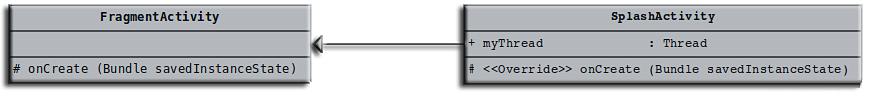
\includegraphics[scale=0.45]{Splash_class_diagram2.png}
\caption{Intro Screen Class Diagram}
\end{figure}

\begin{flushleft}
It is a class that provides Bluetooth access to the Bluetooth feature of the phone with the help of Bluetooth adapters and makes some kind of communication with the Arduino Bluetooth via the Sockets.
\end{flushleft}
\begin{figure}[h]
\centering
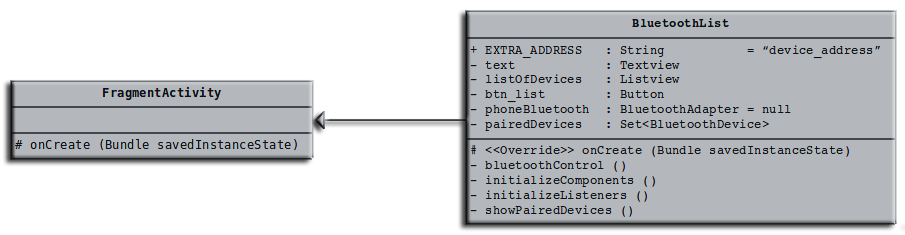
\includegraphics[scale=0.45]{Bluetooth_class_diagram2.png}
\caption{Bluetooth Class Diagram}
\end{figure}

\begin{flushleft}
This one contains classes that control the camera, including  video stream. Basically, everything is managed from the MjpegStream, it’s a view specialized to deal with Mjpeg video stream format, because Android doesn’t support natively this format.
\end{flushleft}
\begin{figure}[h]
\centering
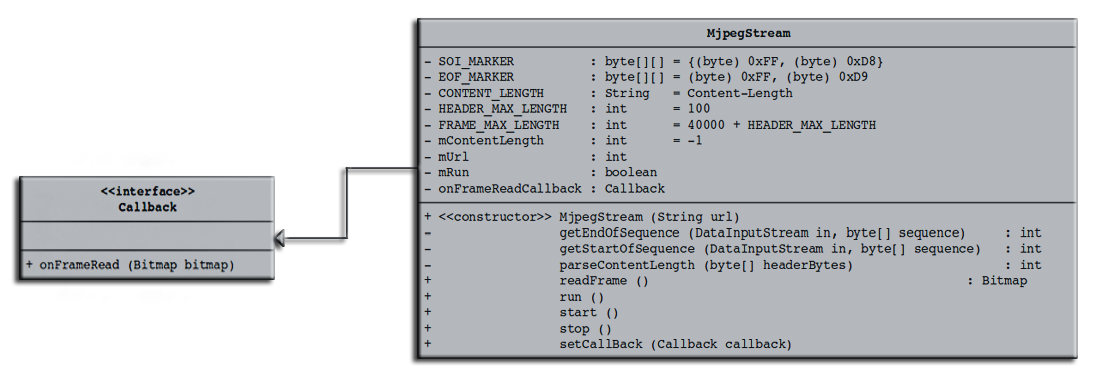
\includegraphics[scale=0.40]{Camera_class_diagram2.png}
\caption{Camera Class Diagram}
\end{figure}

\pagebreak

\begin{flushleft}
This class contains all classes in relationship with the car. The Car class is basically a controller for the car, it’s this class that will control the direction via bluetooth sockets and monitor the live video stream.
\end{flushleft}
\begin{figure}[h]
\centering
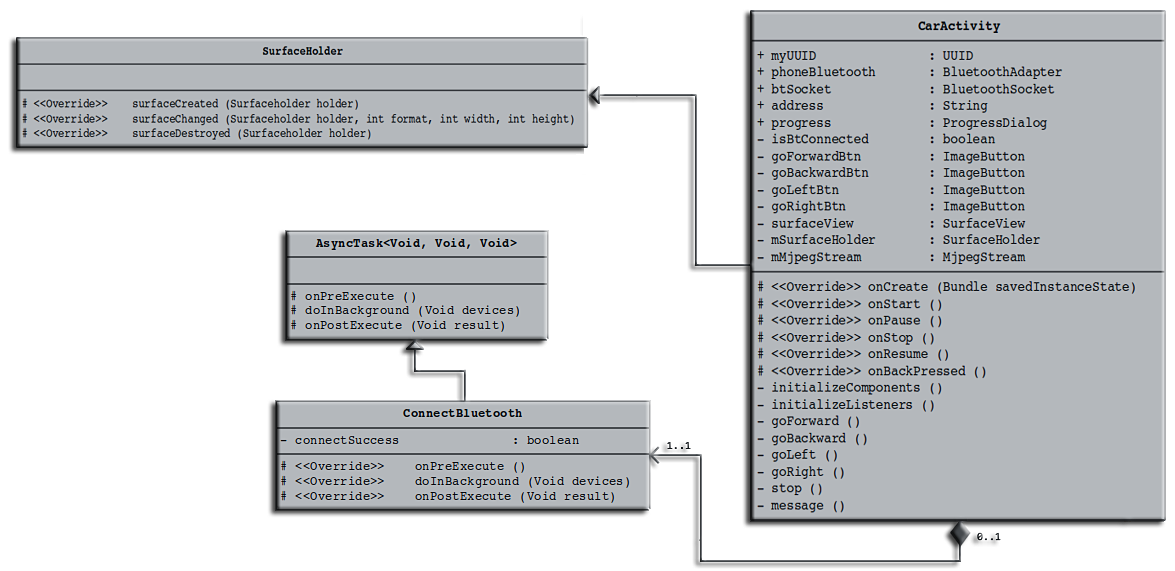
\includegraphics[scale=0.45]{Car_class_diagram2.png}
\caption{Car Activity Class Diagram}
\end{figure}

\pagebreak

\subsection{Use Case Diagram}
\begin{flushleft}
To describe the system functionalities, we use the UML Use case diagrams. The Use Cases diagrams illustrated below show the actors that show also which kind of action they can use.\\
\vspace{0.20cm}
This is the first version of the system, which can basically only move, the details about all the possible movements are described too.
\end{flushleft}
\begin{figure}[h]
\centering
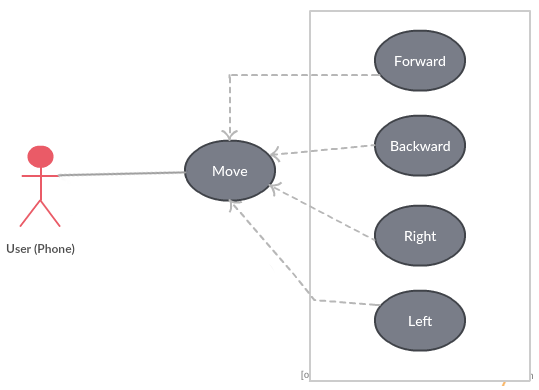
\includegraphics[scale=0.49]{RobotUML_V1.png}
\caption{Use Case - Version1}
\end{figure}

\vspace{0.20cm}
\begin{flushleft}
The second version is a major release of the system because we will reach our goal that is to have a video stream on the phone and control the car almost in real time with good performances.
\end{flushleft}
\begin{figure}[h]
\centering
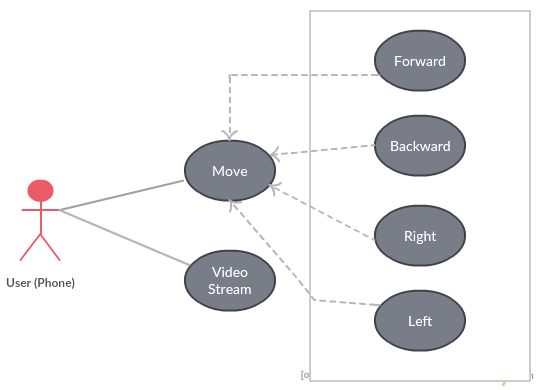
\includegraphics[scale=0.49]{RobotUML_V2.png}
\caption{Use Case - Version2}
\end{figure}

\pagebreak


%%%%%%%%%%%%%%%%%%%%%%%%%%%%%%%%%%%%%%%%%%%%%%%%%%
% SECTION
%%%%%%%%%%%%%%%%%%%%%%%%%%%%%%%%%%%%%%%%%%%%%%%%%%
\section{Conclusion}
\begin{flushleft}
Everything that is smart makes our life easier and more meaningful. Thanks to Arduino Technology, there are now so many systems that make people's lives easier and almost inventive, which is impossible to catch up with. In this project, which is considered to be my thesis, I accomplished to design my own car using Arduino and to use it in mobile environment and watch it.\\
\vspace{0.25cm}
Of course, we need communications to activate these clever things. I used Bluetooth and WIFI technologies that is supported by smartphones.\\
\vspace{0.25cm}
I have learned many things in several parts, hardware or software, even project management, this project helped me, to better understand the communication with hardware and software. I am used to develop software and I am not used to deal with hardware, it’s also really complicated many information and documentation to read, to be aware of. You cannot really break software, it doesn’t happen often, but it’s really easy to break hardware for instance, I discovered that.\\
\vspace{0.25cm}
Managing a stand-alone project; It is very difficult to be both a manager and an employee of the project. During this process, I am really tired and confused. However, I have completed the project successfully and in the most efficient way.
\end{flushleft}

\vspace{0.3cm}

%\subsection{Limitations of the system}
%\begin{flushleft}
%The system has some limitations. We suppose be able to control the car in about 10 meters range before the Wi-Fi signal shutdown.\\
%\vspace{0.25cm}
%We designed the application to use video stream. But we could have some limitations using the camera that could be not powerful enough for live stream, or the Wi-Fi, which could be not fast enough for transmit the live stream.\\
%\vspace{0.25cm}
%The car embedded a battery 9V. The user will need to charge or change it from time to time.
%\end{flushleft}

%\vspace{0.4cm}

\subsection{User profile}
\begin{flushleft}
The users that will be play with the system could be child or adults, they just have to know how to use a smartphone, launch an application and push some buttons. There is no really limitation about the age while they know how to use the phone.
\end{flushleft}

\pagebreak

\subsection{Strengths and weaknesses}
\subsubsection{Strengths}
\begin{itemize}
\item The project works, we are able to do what we wanted.
\item The source code for both Android and Arduino is commented, well explained and documented with external documents.
\item All the source code and the documentation are available for future usages for other people and free. (Git)
\item Good and speed video stream.
\item With the video streaming width designed to fill the user's phone screen, the user will be able to control the car comfortably.
\item It connects to Bluetooth without difficulty and never breaks unless we are away from a certain distance.
\end{itemize}

\subsubsection{Weaknesses}
\begin{itemize}
\item The product needs two separated power sources.
\item Sometimes WiFi can shut down automatically. In this case, the video is freezing because WiFi is off.
\item Really short range with video stream. (~8 meters)
\end{itemize}

\vspace{0.4cm}

\subsection{Suggested improvements (Future of system)}
\begin{itemize}
\item Use external antenna for greater range.
\item Use only one source of power, so use the big battery used by the motor for both motor and Arduino using the regulator.
\item Study and fix bugs on the applications.
\item Improve the Android application to be able to get the video stream and the car control after lost them (out of range) automatically.
\item Add sounds to warn the user on some events such as “out of range”, “video lost”, etc.
\item Improve the application with new modules such as proximity detection using sensor.
\item Improve Android application with a different way to control the car using sensors instead of buttons and propose the choice to the user between both.
\item Some sensors of the Arduino can be added to bring joy to the car. \textit{(honk-buzzer, distance-ultrasonic, headlights-lamp sensor etc.).}
\end{itemize}

\pagebreak



%%%%%%%%%%%%%%%%%%%%%%%%%%%%%%%%%%%%%%%%%%%%%%%%%%
% SECTION
%%%%%%%%%%%%%%%%%%%%%%%%%%%%%%%%%%%%%%%%%%%%%%%%%%
\section{Time Table and Work Schedule}
\subsection{Gantt Chart}
\begin{figure}[h]
\centering
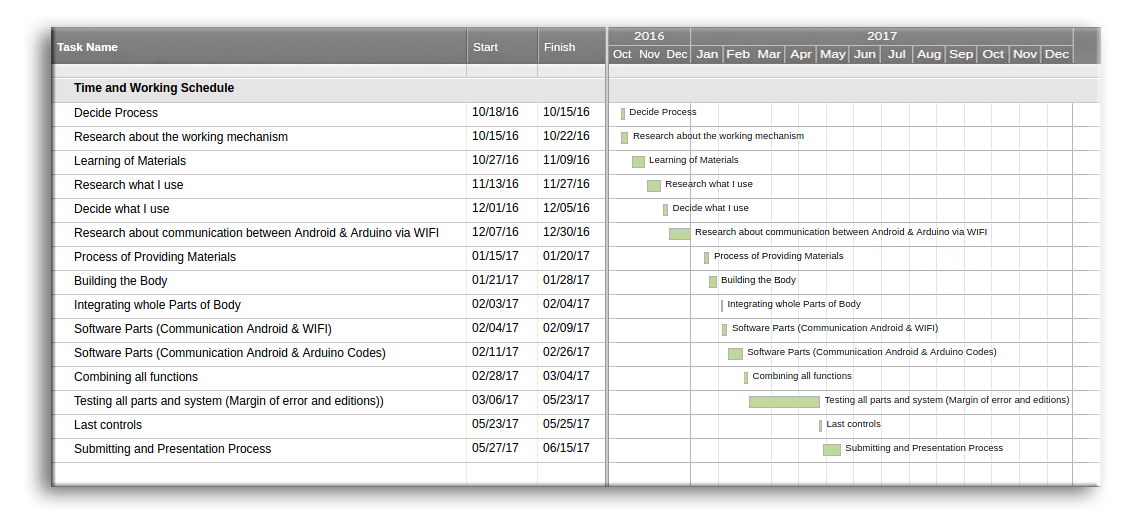
\includegraphics[scale=0.45]{ganttChart.png}
\caption{Time Table and Work Schedule}
\end{figure}

\pagebreak

%%%%%%%%%%%%%%%%%%%%%%%%%%%%%%%%%%%%%%%%%%%%%%%%%%
% SECTION
%%%%%%%%%%%%%%%%%%%%%%%%%%%%%%%%%%%%%%%%%%%%%%%%%%
\section{References}
\begin{itemize}
\item {[Nov2016] - http://electrotech.tv/arduinoya-giris-arduino-nedir-ne-degildir-1bolum/}
\item {[Dec2016] - http://www.robotistan.com/arduino-smd-l298-cift-motor-suucu-shieldarduino-motor-shield\#}
\item {[Jan2017] - http://www.robotiksistem.com/dc\_motor\_ozellikleri.html}
%\item \url {https://gelecegiyazanlar.turkcell.com.tr/konu/arduino/egitim/arduino-201/bluetooth-ile-iletisim}
\item {[Feb2017] - http://android.serverbox.ch/?p=1039}
\item {[Feb2017] - http://stackoverflow.com/questions/3205191/android-and-mjpeg}
\item {[Mar2017] - http://forum.arduino.cc/}
\item {[Mar2017] - https://sites.google.com/site/androidhowto/how-to-1/display-a-web-page}
\item {[April2017] - http://www.bluecove.org/bluecove/apidocs/javax/bluetooth/UUID.html}
\item {[April2017] - http://stackoverflow.com/questions/4032391/android-bluetooth-where-can-i-get-uuid}

\end{itemize}

\end{document}